\section{Results}

\subsection{Training and Model Performance}

We trained the model for 100 epochs using a learning rate of 0.01, a momentum of 0.9, and a weight decay of 0.0005. The final model yields 92.16\% accuracy on the test dataset.

\subsection{Prediction Examples}

Figure~\ref{fig:prediction-examples} shows some examples of images that were being tested and the output that the model predicted. The first row shows the images that are correctly predicted. The second row are images with people wearing masks, but our model falsely predicted that they were not wearing masks. The third row are images of people not wearing masks. However, our model incorrectly predicted that they were wearing masks.

Based on the examples here, we noticed that the images that were correctly predicted tend to have the following characteristics: (1) the human faces are large in the frame, (2) the face part and mask part are easily distinguishable, and (3) there is not much going on in the background.

On the opposite side, images that were incorrectly predicted might contain some of these characteristics: (1) there are variations of color and pattern on the masks, (2) images contain accessories and/or facial hair, which make the model misassociate them with the masks, and (3) the mask is not easily distinguishable from the face.

\begin{figure}
  \caption{
    examples of images that were used to test the model. The first row are images that the model predicted correctly. The second row and the third row are images that the model incorrectly predicted.
  }
  \label{fig:prediction-examples}
  \centering
  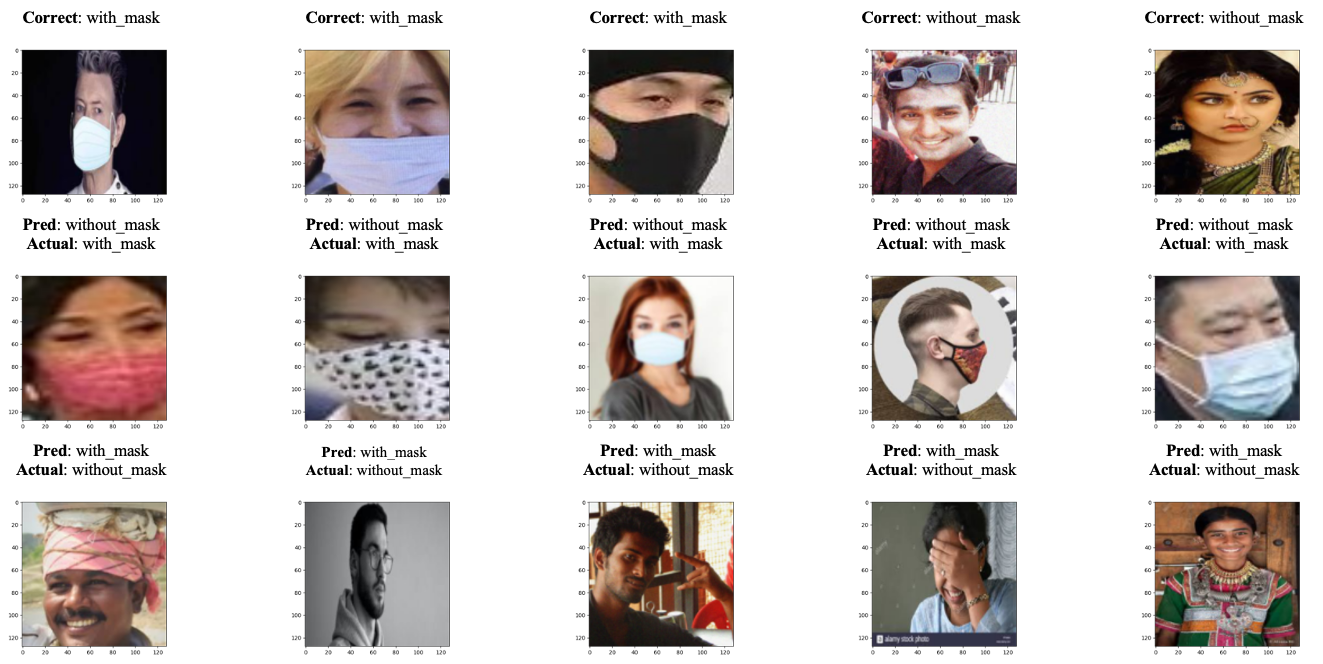
\includegraphics[width=300px]{figures/prediction-examples.png}
\end{figure}

\subsection{Output Layer Visualization}

As the model incorrectly predicted some images, we were curious about the cause of these incorrect predictions.
So, we extracted and visualized the output of the first ReLU layer to see the pattern of what pixels were activated.
In other words, we wanted to know what features our model captured from the images.
Starting from a correctly predicted image (Figure~\ref{fig:output-correct}), we can see that some channels either activate the face part or the mask part.
So, the model can distinguish between the two parts.
Furthermore, we can see that our model can capture the eyes of the humans in the images.
On the other hand, our model cannot capture some of these features in the incorrectly classified images.
In the first incorrectly classified example (Figure~\ref{fig:output-incorrect-1}), our model could not find the clear boundaries between face and mask.
In the second incorrectly classified example (Figure~\ref{fig:output-incorrect-2}), our model could not capture the eyes of the humans in the image.
In the third incorrectly classified example (Figure~\ref{fig:output-incorrect-3}), our model activated the parts of the image that were not the human face.


\subsection{Camera Application}
Our camera application captures video of human faces.
It then processes the video in real-time, frame by frame, by classifying if a human in the frame is wearing a mask or not.
Our camera application does well when the human face is close to the camera (Figure~\ref{fig:camera-correct}).
However, when the human face is far away or when the background of the video has too many objects (Figure~\ref{fig:camera-incorrect}), our model becomes inaccurate.
One future improvement in response to this problem is that we would like to cut out only the human face part of the image before classifying it.
With this improvement, the background of the video becomes irrelevant and will improve the accuracy of our application.
